\selectlanguage{english}%

\chapter{\label{chap:Data-and-analysis}Data and analysis}

This chapter explains our research methodology and results in details.
We begin by explaining the framework of our methods, that consists
of several steps in order to get our results. By the end of this chapter,
we present the results of our analysis to answer the research questions
that we explained in \autoref{chap:research-questions}.


\section{\label{sec:Research-Methodology}Research Methodology}

As we illustrate in \autoref{fig:Research-methodology-diagram}, we
processed our data into several steps. After, we collect the data
from a security organization in the form of suspected phishing email
reports, we performed a data selection that consists of selecting
8444 raw emails into 207 unique phishing emails. The selection process
can be found in \autoref{sub:Selection}. In the next step, we executed
data classification into the variables that we established in \autoref{sub:variables}
so that we could reconstruct into SPSS readable dataset. Lastly, we
conduct statistical analyses to answer our hypotheses.

\begin{figure}[H]
\begin{centering}
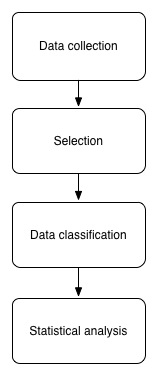
\includegraphics[scale=0.7]{gfx/methodology_diagram}\protect\caption{\label{fig:Research-methodology-diagram}Research methodology diagram}

\par\end{centering}

\selectlanguage{american}%
\selectlanguage{american}%
\end{figure}



\subsection{Data collection}

The data was obtained from an organization based in Netherlands that
handles reports on online crime and fraud including phishing in the
form of phishing emails, which were reported between August 2013 and
December 2013. The data consists of 8444 suspected phishing emails
in total that will be selected and classified in the following sections.


\subsection{\label{sub:Selection}Selection}

\begin{figure}[H]
\selectlanguage{american}%


\selectlanguage{english}%
\begin{centering}
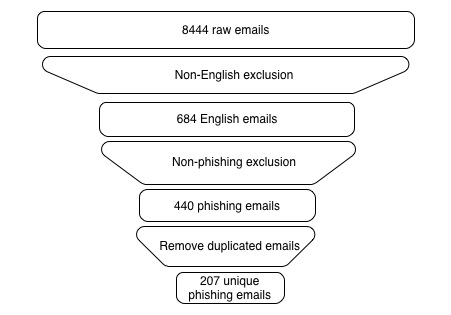
\includegraphics[scale=0.7]{gfx/selection}\protect\caption{\label{fig:Selection-diagram}Selection diagram}

\par\end{centering}

\selectlanguage{american}%
\selectlanguage{american}%
\end{figure}


The selection process consists of non-English exclusion, non-phishing
exclusion and removing duplicated emails. \autoref{fig:Selection-diagram}
illustrates the selection process.


\subsubsection{Non-English exclusion}

By manually inspecting each of suspected phishing email, we can separate
the emails based on the languages. These languages consist of English,
Dutch and other languages. The raw data was sorted by the subject
to help the separation process easier. This process gave the following
results:
\begin{itemize}
\item 7756 suspected phishing in Dutch language
\item 684 suspected phishing in English language
\item 4 suspected phishing in Other languages
\end{itemize}
We excluded the suspected phishing emails in non-English languages
because our proficiency of non-English languages is not sufficient.
More detail on why we excluded the emails with non-English languages
can be found in \autoref{sec:Limitation} and \autoref{sec:Future-work}. 


\subsubsection{Non phishing exclusion}

From 684 suspected phishing emails in English group, we exclude the
non-phishing emails by categorized them into Phishing, Legitimate
and Others groups. The phishing group consists of the emails that
were indeed phishing. The legitimate group consists of legitimate
emails. The others group contains spam emails that represent commercial
advertisements and the emails that have no content, for instance,
when the content has been removed before it was forwarded. 

This process gave the following results:
\begin{itemize}
\item 440 Phishing
\item 18 Legitimate
\item 226 Others 
\end{itemize}
Interestingly, based on the result of the categorization process,
we found 18 legitimate emails that were mistakenly reported as phishes
(i.e. false positives). This suggests that although there are only
18 false positives, misinterpretation of a fraudulent email among
the reporters is still occurred.


\subsubsection{Removing duplicated emails}

From this point we would only code 440 phishing emails to an excel
sheet with necessary variables so that we could convert the excel
sheet into SPSS readable file. Our aim was to analyze only the unique
phishing emails, so that the dataset would not be redundant. Duplicated
emails in our dataset defined as having exactly the same text in the
entire body of the emails. To find duplicated phishing emails, we
conducted the following steps:
\begin{enumerate}
\item Sorting the 440 emails by the subject, to show which email that has
the same subject.
\item Manually investigate each email that has other emails with the same
subject to make sure all the text in the entire body is exactly the
same. If not we discriminated it.
\item Sometimes duplicated emails have slightly different subject. To find
more duplicated emails, we search based on random phrase from the
body.
\item If other emails found, we manually investigate each email to make
sure they have exactly the same text in the entire body.
\item We indicate the number of duplicated emails in ``CounterSameContents''
variable that we will explain in \autoref{sub:variables}.
\end{enumerate}
These steps gave 207 unique phishing emails.


\subsection{Data Classification}

We classify our data accordingly into our variables so that we can
have a usable dataset which can be analyzed. We put either 0 or 1
in our variables except Mail ID, Timestamps, CountMessageReporter,
Target and Reason variables. For example, when a phishing email has
a PDF attachment, we put value ``1'' in our ``PDFattachment''
variable. Similarly, if phishing email has a hyperlink in the content,
we put value ``1'' in our ``ContainHyperlink'' variable. As we
want to analyze our dataset based on Cialdini's persuasion principles,
it is important for us to explain our rationale and conception on
Cialdini's principles. We will explain our variables and persuasion
conception in the following sections.


\subsubsection{\label{sub:variables}Variables and concepts}

As we study phishing email properties in \autoref{sub:Stop-phishing-at},
variables are need to be established to code our dataset into, so
that we will be able to conduct the statistical analysis in the SPSS
application. Based on our findings in the literature survey on phishing
email properties, 23 Variables were created as part of the methodology
processes prior our data classification. Generic properties are depicted
by the structural properties in phishing emails except persuasion
principles. The variables are explained in the following list:
\begin{enumerate}
\item \emph{Mail ID} : Unique ID {[}Scale measurement{]}
\item \emph{Timestamps}: Implies the date and time when the email is being
reported {[}Scale measurement{]}
\item \emph{Attachments:} Indicates whether the phishing email has an attachment(s),
if so, what kind of attachment

\begin{enumerate}
\item PDF {[}0 = No, 1 = Yes{]}
\item ZIP {[}0 = No, 1 = Yes{]}
\item HTML {[}0 = No, 1 = Yes{]}
\end{enumerate}
\item \textit{Instructions}: Implies the inquiry by the phishers in the
contents

\begin{enumerate}
\item ReqOpenAttachment; A request to respond by opening an attachment(s)
{[}0 = No, 1 = Yes{]}
\item ReqClickLink; A request to respond by clicking URL(s) {[}0 = No, 1
= Yes{]}
\item ReqEmailReply; A request to respond by email reply {[}0 = No, 1 =
Yes{]}
\item ReqCallingByPhone; A request to respond by calling through phone {[}0
= No, 1 = Yes{]}
\end{enumerate}
\item \emph{Contents}: Indicates what elements are included in the body

\begin{enumerate}
\item ContainHyperlink {[}0 = No, 1 = Yes{]}
\item UseHTML {[}0 = No, 1 = Yes{]}
\item IncludesImage {[}0 = No, 1 = Yes{]}
\end{enumerate}
\item \emph{HiddenURL}: Specifies whether a phishing email has a hidden
URL(s) {[}0 = No, 1 = Yes{]}
\item \emph{CountMessageReporter}: A counter where the reporter includes
an extra information with the minimum value 0. For instance, A reporter
said ``Geen spam, maar phishing!'', we put a value 1 in this variable
{[}Nominal measurement{]}
\item \emph{Target}: Determined the target institutions

\begin{enumerate}
\item TargetType {[}Values can be seen in \autoref{tab:Target-classification}{]}
\end{enumerate}
\item \emph{Reason}: Implies the reason why the unsuspected victim must
grant the phisher's request

\begin{enumerate}
\item ReasonType {[}Values can be seen in \autoref{tab:Reason-classification-1}{]}
\end{enumerate}
\item \emph{Cialdini's Principles}: Specifies what principle(s) the phishing
email signifies. 

\begin{enumerate}
\item Reciprocation {[}0 = No, 1 = Yes{]}
\item Consistency {[}0 = No, 1 = Yes{]}
\item SocialProof {[}0 = No, 1 = Yes{]}
\item Likeability {[}0 = No, 1 = Yes{]}
\item Authority {[}0 = No, 1 = Yes{]}
\item Scarcity {[}0 = No, 1 = Yes{]}
\end{enumerate}
\item \emph{CounterSameContents}: A number that specifies how many emails
are duplicated. The minimum value of this variable is 1, which indicates
a unique email. For example, value 2 indicates that there is (2-1)
duplicated email with the same text in the body, value 3 means there
are (3-1) duplicated emails. The reason to have this variable was
for us to make sure we can track back from 207 unique phishing emails
to 440 phishing emails.
\end{enumerate}
We have established the variables based on the phishing email properties.
We also distinguished generic properties and persuasion properties.
The generic properties of a phishing email is effected by these variables:
attachments, requests, contents, hiddenURL, target and reason. On
the other hand, the persuasion properties effected by these variables:
reciprocation, consistency, social proof, likeability, authority and
scarcity.


\subsubsection{\label{sub:cialdini}Cialdini's principles and conception}

Part of our analysis, we tried to analyze phishing emails dataset
based on Cialdini\textquoteright s principles titled \textquotedblleft The
science of persuasion\textquotedblright . The decision making and
the rationale in this process are achieved based our perspective of
Cialdini\textquoteright s principles in the following details.

\emph{Reciprocation}: The norm that obligates individuals to repay
in kind what they have received. Return the favor. Adjustment to smaller
request \cite{cialdini:2001}. When a phisher sends an email containing
a message that perceived as a request or obligation towards the recipient
to \textquotedblleft return the favor\textquotedblright . It might
be natural for an individual to feel \textquotedblleft obligated\textquotedblright{}
to return the favor for things or information that he/she is given
and is deemed to be valuable. For example in the phishing email context,
when PayPal has detected there are suspicious activities on our account,
we sometimes believe that PayPal has done a good job in detecting
security risk on their system and we feel \textquotedblleft obligated\textquotedblright{}
to return the favor of that valuable information. Another example,
if the sender gave the information that they have added \textquotedblleft extra
security\textquotedblright{} on their system so that we also feel
obligated to grant their request. 

\emph{Consistency}: Public commitment. When people become psychologically
become vested in a decision they have made \cite{workman:2008}. When
a phishing email contains a message that perceived to request recipient\textquoteright s
\textquotedblleft consistency\textquotedblright{} on a decision they
have made. For example in the phishing email context, when a hotel
agent asks us to review the payment details of our reservation that
we have previously made, we might feel committed or agreed to review
the payment details that has been given. Another example, if Facebook
gave a link to change your password that you requested previously
to change it. It might be not applicable to those who are not requesting
password previously, but we believe it will impact to those who are
committed to change the password previously. 

\emph{Social proof}: It occurs when people model the behavior of their
peer group, role models, important others or because it is generally
\textquotedbl{}fashionable\textquotedbl{} \cite{workman:2008}. For
example, when someone tells us that there are a hundreds of other
people who use particular system, so we might want to agree to use
it as well just because a lot of other people use it as well. Another
example, when Facebook give information that someone wants to be our
friend, and we knew who that someone is. We might tend to follow that
request and click the link to accept the request. 

\emph{Likeability}: It occurs when people trust and comply with requests
from others who they find attractive or are perceived as credible
and having special expertise or abilities such as sports figures or
actors they like \cite{workman:2008}.When a phishing email contains
a message that attracts recipient to comply the sender\textquoteright s
request based the reference on something or someone that likeable
for the recipient. Cialdini \cite{cialdini:2001} identified that
people usually \textquotedblleft trust those they like\textquotedblright .
For example, if someone is asking us to download and listen to a music
that Michael Jackson made, we might be attracted to download and listen
to it just because we happen to love Michael Jackson music. It is
like someone is asking us to watch a concert and he/she said, \textquotedblleft Coldplay
will be there\textquotedblright , if we are devoted fan of Coldplay,
we might find it very interesting. Another example, when a sender
gives compliments to us or committed to help us to safeguard our account
from the hackers, we tend to think that the sender cares about our
safety, which is good for us, and consequently it might attract us
to comply with the sender\textquoteright s request. 

\emph{Authority}: It can be used to engender fear, where people obey
commands to avoid negative consequences such as losing a privilege
or something of value, punishment, humiliation or condemnation \cite{workman:2008}.
When a phishing email contains logo or image or signature or anything
that looks like legitimate institutions. It can be used to makes it
look trustworthy so that the recipient might accept and obey the sender\textquoteright s
request. For example, when an email is presenting somehow authentic
looking signature like \textquotedblleft Copyright 2013 PayPal, Inc.
All rights reserved\textquotedblright{} or PayPal logo. Cialdini \cite{cialdini:2001}
suggests that authoritative persuasion could be achieved by only presenting
\textquotedblleft aura of legitimacy\textquotedblright . Another example,
when the content of the email stated that it is from \textquotedblleft System
Administrator\textquotedblright{} asking for password update. It would
be not authoritative if only random people asking us to change our
password. 

\emph{Scarcity}: Based on the principle of reactance, where people
respond to perceived shortages by placing greater psychological value
on perceived scarce items \cite{workman:2008}. When a phishing email
contains a message that tells a recipient to react or respond to scarce/turns-into
scarce items or things or privileges. For example in the phishing
email context, if a sender tells us that he/she will suspend/deactivate/limit
our account if not respond to his/her request, we might want to respond
to their request because we are worried we will not able to access
our account again or in other words our account become scarce or limited.

\begin{figure}[H]
\begin{centering}
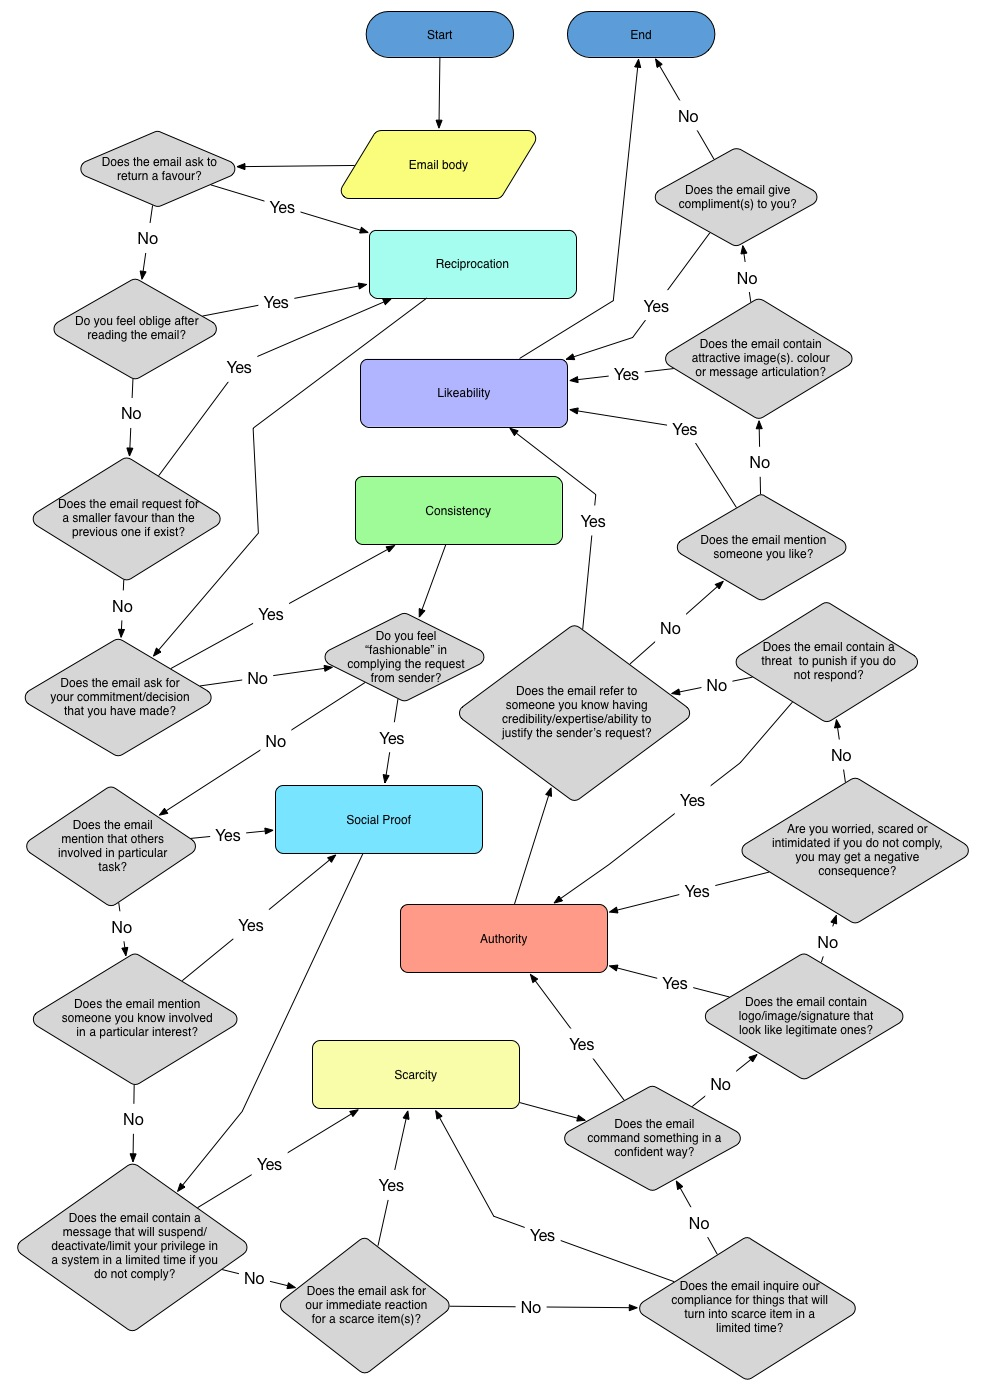
\includegraphics[scale=0.4]{gfx/pseudo-cialdini-2}
\par\end{centering}

\protect\caption{\label{fig:Flowchart-cialdini}Integration pseudo-code of Cialdini's
principles}
\end{figure}


We have made a flowchart%
\footnote{Shapes and lines were created based on http://www.rff.com/how\_to\_draw\_a\_flowchart.htm%
} in \autoref{fig:Flowchart-cialdini} that illustrates our analysis
of the dataset based on Cialdini's principles. 


\subsection{Statistical analysis}

In the previous section, we have described the framework of our methodology
in considerable details. Until data classification, we have used Microsoft
Excel to code our data. To perform the analyses, we transform the
data into SPSS readable file. We initially record our data in 23 variables
which could be expanded depending on our analyses, such as selecting
cases which have all instructions or selecting a specific target sector.

The data has been analyzed by quantitative analysis from mainly three
different viewpoints; general properties characteristics, persuasion
principles characteristics and their relationships. We used frequency
analysis to answer questions related to occurrences. For instance,
we used frequency analysis to answer the most targeted institution
in \autoref{chap:research-questions}. Furthermore, we used Pearson
chi-square to test our hypotheses to discover if there is a significant
relationship between two variables. If the resulted p-value is less
than 0.05, 0.01, or 0.001, we are confident 95\%, 99\% and 99.9\%
respectively that the two chosen variables are having a significant
relationship. By combining frequency analysis and chi-square test,
we will see how they can answer our research questions in the next
section. As our data is not continuous (i.e. interval or ratio) but
nominal (i.e. categorical), we do not analyze our data by Pearson
correlation. However, to test the strength of association involves
nominal variables, the appropriate measurements are using phi and
Cramer's V. Phi is used for 2 by 2 table and Cramer's V can be used
for more than 2 by 2 table. Since our data will be analyzed on 2 by
2 table, therefore, Phi measurements will be used. Values close to
0 indicate a very weak relationship, and values close to -1 or +1
indicate a very strong negative or positive relationship respectively.


\section{Results}

In this section, we elaborate on the results we have obtained through
our analyses. We begin this section by describing the frequency analyses
of the general structural properties and persuasion principles. We
then describe the relationship analysis between the general structural
properties and the persuasion principles. We conclude the section
by mentioning the results related to persuasion principles used in
phishing emails.

We find that 36.2\% of the total phishing emails have attachment(s)
included within its content, On the other hand, 63.8\% of them do
not have attachment. In addition, we also look at what types of attachment
does one has. Of the total emails having attachment, we find that
4\% have PDF attachment, 78.7\% have ZIP attachment, 12\% have HTML
attachment and 5.3\% of them have the attachment(s) removed before
the emails were forwarded. We are not sure what type of attachments
they have, but we determined that the attachment element is still
there if the request to open attachment within its content is presence.
For example, an email dated December 20th 2013 11:29am, it was said
in the email's body ``...we have send the attached as a secure electronic
file'', however, it did not attach anything. Therefore, we suspected
that it was removed by antivirus software. \autoref{tab:Attachment(s)-analysis}
illustrates our finding on attachment variables. 

When we look deeper, we find that there is a significant relationship
between ZIP file and Attachment variable, a chi-square test resulted
in $X^{2}(1)=145.236,p<0.001$. Similarly, there is a significant
association between HTML file and Attachment variable with a chi-square
test resulted in $X^{2}(1)=16.560,p<0.001$. However when we test
the relationship between PDF and attachment, the significancy level
is not as strong as ZIP and HTML, $X^{2}(1)=5.358,p=0.021$.

\begin{table}[h]
\begin{centering}
\begin{tabular}{ccc}
\toprule 
Type of attachment & \textsc{Frequency} & \textsc{Percent}\tabularnewline
\midrule
\midrule 
{\footnotesize{}ZIP } & {\footnotesize{}59} & {\footnotesize{}78.7}\tabularnewline
\midrule 
{\footnotesize{}HTML } & {\footnotesize{}9} & {\footnotesize{}12}\tabularnewline
\midrule 
{\footnotesize{}Removed } & {\footnotesize{}4} & {\footnotesize{}5.3}\tabularnewline
\midrule 
{\footnotesize{}PDF} & {\footnotesize{}3} & {\footnotesize{}4}\tabularnewline
\midrule 
\textsc{\footnotesize{}Total} & {\footnotesize{}75} & {\footnotesize{}100}\tabularnewline
\bottomrule
\end{tabular}\protect\caption{\label{tab:Attachment(s)-analysis}Attachment analysis}

\par\end{centering}

\selectlanguage{american}%
\selectlanguage{american}%
\end{table}


\ 

When we look at what are the instructions or requests used in the
dataset. We find 202 emails or 97.6\% of all total reported phishing
emails with clear instructions; whether it requests to click URL(s),
request to open attachment, request to reply by email or request to
respond by phone calling. 2.4\% of the total emails do not contain
a clear or unclear instructions to the recipients, for instance, at
24 November 2013 on 19:59, the email only include attachment(s) without
asking to open it. However, with the subject of ``Payrolls reports''
we have the impression that this is a targeted phishing email, which
means it only aims a small audience as the recipients, usually a certain
institution. More example, at 15 august 2013 on 17:38, it contains
HTML based email that suggests a recipient to check the interesting
pages on Facebook. However, we did not find any instruction to click
on URL nor other instructions. Apart from the instruction to click
URL(s), we find that 37.2\% of the total phishing emails request to
open attachment, 52.7\% of them request to click URL(s), 16.9\% request
for email reply and 4.3\% request to call by phone. Moreover. One
single email can request multiple requests. If we look deeper, we
have 8 valid emails or 3.9\% of all emails which have both request
to open attachment and request to click URL. However, we do not find
any email which request all instructions in the content. \autoref{tab:Methods-analysis}
illustrates our findings in respect of requests are used. In addition,
of all phishing emails which have clear instructions, 54\% request
to click URL(s), 38.1\% request to open attachment(s), 17.3\% request
for email reply and 4.5\% request to respond by phone calling.

\begin{table}[h]
\begin{centering}
\begin{tabular}{ccc}
\toprule 
\textsc{\small{}Request} & \textsc{\small{}Frequency} & \textsc{\small{}Percent}\tabularnewline
\midrule
\midrule 
{\small{}click URL} & {\small{}109} & {\small{}52.7}\tabularnewline
\midrule 
{\small{}open Attachment(s)} & {\small{}77} & {\small{}37.2}\tabularnewline
\midrule 
{\small{}Email Reply} & {\small{}35} & 16.9\tabularnewline
\midrule 
{\small{}call by phone} & {\small{}9} & {\small{}4.3}\tabularnewline
\bottomrule
\end{tabular}\protect\caption{\label{tab:Methods-analysis}Request analysis of all total emails
(one email can contain more than one instructions so the total here
does not sum up to 100\%)}

\par\end{centering}

\selectlanguage{american}%
\selectlanguage{american}%
\end{table}


\ 

As we discussed before, we have also analyzed the content of phishing
emails in our corpus. We look at whether it has URL(s), using HTML
code or includes image(s) within its content. We find that 60.4\%
have URL(s) while 39.6\% do not have URL. 66.2\% of the emails use
HTML code while 33.8\% do not use HTML code within its content. We
find 35.3\% of them include image(s) while 64.7\% do not include image.
\autoref{tab:Content-analysis} highlights our findings in respect
of content analysis. The percentage depicted of all total emails.
If we look further of all emails which utilized HTML, 120 emails or
87.6\% of them have provided URL(s) and 73 or 53.3\% of them include
image(s). Furthermore, of all 73 emails that include image, 67 emails
or 91.8\% of them have provided URL(s). Based on this result, we know
that one variable overlap with other variables. Therefore, the total
percentage does not sum up to 100\%.

\begin{table}[h]
\centering{}%
\begin{tabular}{ccc}
\toprule 
\textsc{\small{}Content} & \textsc{\small{}Frequency} & \textsc{\small{}Percent}\tabularnewline
\midrule
\midrule 
{\small{}utilizing HTML} & {\small{}137} & 66.2\tabularnewline
\midrule 
{\small{}URL presence} & {\small{}125} & 60.4\tabularnewline
\midrule 
{\small{}include Image} & {\small{}73} & {\small{}35.3}\tabularnewline
\bottomrule
\end{tabular}\protect\caption{\label{tab:Content-analysis}Content analysis of all total emails
(one email can contain more than one content variables so the total
here does not sum up to 100\%)}
\end{table}


\ 

When we look at target classification table in \autoref{tab:Target-analysis},
we find that financial sector is the most targeted sector and ISP
is the least common target in our corpus. Furthermore, E-Commerce/retails,
administrator and government allocated in the second, third and fourth
respectively as the most targeted sectors. When we look deeper at
the detailed list of target brand, we find PayPal as a financial institution
is the highest frequency at 37.2\% of the total financial targeted
emails. We find Bank of America contributes 6.4\% and American Express
5.1\%. Furthermore, Visa contributes 5.1\% and Western union contributes
3.8\%. Other financial institutions contributes below 3\% of frequency.
\autoref{fig:Detailed-of-financial} illustrates the detailed target
brand of financial sector.

As one email does not have more than 1 targeted sector, therefore
the total sums up to 100\%. Note that, we initially had 92 targets
in our corpus and we had to classify them into 10 target types in
our data classification.

\begin{table}[h]
\begin{centering}
\begin{tabular}{ccc}
\toprule 
\textsc{\small{}Target} & \textsc{\small{}Frequency} & \textsc{\small{}Percent}\tabularnewline
\midrule
\midrule 
{\small{}Financial} & {\small{}78} & {\small{}37.7}\tabularnewline
\midrule 
{\small{}E-commerce/retails} & {\small{}40} & {\small{}19.3}\tabularnewline
\midrule 
{\small{}Administrator} & {\small{}30} & {\small{}14.5}\tabularnewline
\midrule 
{\small{}Government} & {\small{}14} & {\small{}6.8}\tabularnewline
\midrule 
{\small{}Non-existence/individual} & {\small{}13} & {\small{}6.3}\tabularnewline
\midrule 
{\small{}Social media} & {\small{}11} & {\small{}5.3}\tabularnewline
\midrule 
{\small{}Postal service} & {\small{}9} & {\small{}4.3}\tabularnewline
\midrule 
{\small{}Travel agency} & {\small{}5} & {\small{}2.4}\tabularnewline
\midrule 
{\small{}Industrial} & {\small{}5} & {\small{}2.4}\tabularnewline
\midrule 
{\small{}ISP} & {\small{}2} & {\small{}1}\tabularnewline
\midrule
\midrule 
\textsc{\small{}Total} & \textsc{\small{}207} & \textsc{\small{}100}\tabularnewline
\bottomrule
\end{tabular}
\par\end{centering}

\begin{centering}
\protect\caption{\label{tab:Target-analysis}Target analysis}

\par\end{centering}

\selectlanguage{american}%
\selectlanguage{american}%
\end{table}


When we look at what reasons are used in \autoref{tab:Reason-classification},
we find that 48.8\% of the total emails are account related, 25\%
are financial reason and 11.1\% are document related reason. In addition,
only 9.7\% are product/services reason and only 4.8\% are social reason.
When we look further, account related reason consists of security
risk which contributes 28.7\% of account related emails. Account related
reason also consists of system upgrade, new system requirement and
account expiration which contribute below 11\%. This suggests that
account related is the most common pretext to manipulate recipients
in our corpus while social is evidently the least common pretext.
\autoref{fig:Detailed-account-related} illustrates the detailed list
of account related reason.

\begin{table}[h]
\centering{}%
\begin{tabular}{ccc}
\toprule 
\textsc{\small{}Reason} & \textsc{\small{}Frequency} & \textsc{\small{}Percent}\tabularnewline
\midrule
\midrule 
{\small{}Account related} & {\small{}101} & 48.8\tabularnewline
\midrule 
{\small{}Financial incentive} & {\small{}53} & 25.6\tabularnewline
\midrule 
{\small{}Document related} & {\small{}23} & {\small{}11.1}\tabularnewline
\midrule 
Product/services & 20 & 9.7\tabularnewline
\midrule 
Social  & 10 & 4.8\tabularnewline
\midrule
\midrule 
\textsc{\small{}Total} & 207 & 100\tabularnewline
\bottomrule
\end{tabular}\protect\caption{\label{tab:Reason-classification}Reason classification}
\end{table}


\begin{figure}[h]
\selectlanguage{american}%


\selectlanguage{english}%
\begin{centering}
\includegraphics[scale=0.6]{\string"gfx/reasons_detailed_17september2014_bar chart1\string".jpg}\protect\caption{\label{fig:Detailed-account-related}Detailed account related reason
graph}

\par\end{centering}

\selectlanguage{american}%
\selectlanguage{american}%
\end{figure}


We look at the result of persuasion techniques analysis based on Cialdini's
principles with our corpus. As we can see from \autoref{tab:Persuasion-principle-analysis},
we find that 96.1\% of the total phishing emails are using authority
principle, which holds the most used technique in our dataset. Followed
by scarcity principle at 41.1\%. While 21.7\% of the total are using
likeability principle, only 17.4\% of them are using consistency principle.
We find 9.7\% are using reciprocation principle and 5.3\% of them
are using social proof principle. Since authority holds the highest
persuasion technique in our corpus, it is interesting to know why
phishers often use authority as the main technique. Perhaps, most
people do not want to get negative consequences as a result of disobedience
from authoritative figure. Consequently, those people who respond
more obediently to authority more likely to comply with the email's
requests than people who are more skeptical to authoritative figure.
Note that one email can use multiple principles. Therefore, the total
percentage does not sum up to 100\%.

\begin{table}[h]
\centering{}%
\begin{tabular}{ccc}
\toprule 
\textsc{\small{}Cialdini's principles} & \textsc{\small{}Frequency} & \textsc{\small{}Percent}\tabularnewline
\midrule
\midrule 
{\small{}Authority} & 199 & 96.1\tabularnewline
\midrule 
{\small{}Scarcity} & 85 & 41.1\tabularnewline
\midrule 
{\small{}Likeability} & 45 & 21.7\tabularnewline
\midrule 
Consistency & 36 & 17.4\tabularnewline
\midrule 
Reciprocation & 20 & 9.7\tabularnewline
\midrule 
Social proof & 11 & 5.3\tabularnewline
\bottomrule
\end{tabular}\protect\caption{\label{tab:Persuasion-principle-analysis}Persuasion principles analysis}
\end{table}


Based on the result of persuasion principles analysis, we know that
authority principle is the most used principle in our corpus. Now,
we look at the relationship between government and authority principle
to test hypothesis 1. We find that 95.9\% of non-government targeted
emails have authority principle and 4.1\% of them do not impersonate
government nor having authority principle. We find 100\% of government
targeted emails are having authority principle. On the other hand,
we find 93\% of all authority emails are non government targeted email
and 7\% of them are government targeted emails. \autoref{tab:Government-and-authority}
depicted the relationship between government targeted email and authority
principle. Furthermore, of all phishing emails, 6.8\% of them which
have both authority and government targeted sector. A chi-square test
was performed and we find that there is no significant association
between government sector and authority principle, $X^{2}(1)=0.604,p=0.473$.
since p is not less than 0.05, thus we reject hypothesis 1.

\begin{minipage}[t]{1\columnwidth}%
\begin{longtable}{cccc}
\caption{\label{tab:Government-and-authority}Government sector and authority
principle}
\tabularnewline
\toprule 
\textsc{\footnotesize{}Type of Target} & {\footnotesize{}Non-authority} & {\footnotesize{}Authority} & \multirow{1}{*}{{\footnotesize{}N}}\tabularnewline
\midrule 
\multirow{1}{*}{{\footnotesize{}Non-government}} & {\footnotesize{}8} & {\footnotesize{}185} & \multirow{1}{*}{{\footnotesize{}193}}\tabularnewline
\midrule 
\multirow{1}{*}{{\footnotesize{}Government}} & {\footnotesize{}0} & {\footnotesize{}14} & \multirow{1}{*}{{\footnotesize{}14}}\tabularnewline
\midrule
\midrule 
{\footnotesize{}N} & {\footnotesize{}8} & {\footnotesize{}199} & {\footnotesize{}207}\tabularnewline
\midrule
\midrule 
{\footnotesize{}Pearson chi-square} & \multicolumn{3}{c}{{\footnotesize{}0.604}}\tabularnewline
\midrule
\end{longtable}%
\end{minipage}

When we look at the relationship between phishing emails which impersonate
administrator and authority principle to test hypothesis 2. We find
that 96.7\% of administrator targeted emails have authority principle
and 96\% of non-administrator emails have authority principle. On
the other hand, 85.4\% of all authority emails are non administrator
and 14.6\% of them are administrator targeted emails. A chi-square
test was performed and we find that there is no significant relationship
between administrator target and authority principle, $X^{2}(1)=0.027,p=0.870$.
Since p is not less than 0.05, therefore we reject hypothesis 2. \autoref{tab:Administrator-sector-and}
highlights the relationship between administrator sector and authority
principle.

\begin{minipage}[t]{1\columnwidth}%
\begin{longtable}{cccc}
\caption{\label{tab:Administrator-sector-and}Administrator sector and authority
principle }
\tabularnewline
\toprule 
\textsc{\footnotesize{}Type of Target} & {\footnotesize{}Non-authority} & {\footnotesize{}Authority} & \multirow{1}{*}{{\footnotesize{}N}}\tabularnewline
\midrule 
\multirow{1}{*}{{\footnotesize{}Non-administrator}} & {\footnotesize{}7} & {\footnotesize{}170} & \multirow{1}{*}{{\footnotesize{}177}}\tabularnewline
\midrule 
\multirow{1}{*}{{\footnotesize{}Administrator}} & {\footnotesize{}1} & {\footnotesize{}29} & \multirow{1}{*}{{\footnotesize{}30}}\tabularnewline
\midrule
\midrule 
{\footnotesize{}N} & {\footnotesize{}8} & {\footnotesize{}199} & {\footnotesize{}207}\tabularnewline
\midrule
\midrule 
{\footnotesize{}Pearson chi-square} & \multicolumn{3}{c}{{\footnotesize{}0.027}}\tabularnewline
\midrule
\end{longtable}%
\end{minipage}

Now we look at the association between financial sector and scarcity
principle to test hypothesis 3. We find that 39.7\% of all phishing
emails which target financial sector have scarcity principle while
60.3\% do not have scarcity principle. Furthermore, 41.9\% of all
non financial targeted emails have scarcity principle, while 58.1\%
of them do not have scarcity principle. On the other hand, 63.5\%
of scarcity emails is non financial targeted emails, inversely 36.5\%
of them is financial targeted emails. We performed a chi-square test
and we find that there is no significant association between financial
sector and scarcity principle, $X^{2}(1)=0.090,p=0.764$. Since p
is not less than 0.05, thus, we reject hypothesis 3. \autoref{tab:Financial-sector-and}
illustrates the relationship between financial targeted emails and
scarcity principle.

\begin{minipage}[t]{1\columnwidth}%
\begin{longtable}{cccc}
\caption{\label{tab:Financial-sector-and}Financial sector and scarcity principle}
\tabularnewline
\toprule 
{\footnotesize{}Type of Target} & {\footnotesize{}Non-scarcity} & {\footnotesize{}Scarcity} & \multirow{1}{*}{{\footnotesize{}N}}\tabularnewline
\midrule 
\multirow{1}{*}{{\footnotesize{}Non-financial}} & {\footnotesize{}75} & {\footnotesize{}54} & \multirow{1}{*}{{\footnotesize{}129}}\tabularnewline
\midrule 
\multirow{1}{*}{{\footnotesize{}Financial}} & {\footnotesize{}47} & {\footnotesize{}31} & \multirow{1}{*}{{\footnotesize{}78}}\tabularnewline
\midrule
\midrule 
{\footnotesize{}N} & {\footnotesize{}122} & {\footnotesize{}85} & {\footnotesize{}207}\tabularnewline
\midrule
\midrule 
{\footnotesize{}Pearson chi-square} & \multicolumn{3}{c}{{\footnotesize{}0.090}}\tabularnewline
\midrule
\end{longtable}%
\end{minipage}

We look at the association between phishing emails which are targeting
e-commerce/retails and likeability principle to test hypothesis 4.
We find that 20\% of e-commerce/retails targeted emails have likeability
principle. Furthermore, 22.2\% of non e-commerce/retails targeted
emails have likeability principle. On the other hand, only 17.8\%
of all likeability emails are e-commerce/retails targeted emails.
A chi-square test was performed and we find that there is no significant
association between phishing emails targeting e-commerce/retails and
likeability principle, $X^{2}(1)=0.088,p=0.767$. Since p is not less
than 0.05, therefore we reject hypothesis 4. \autoref{tab:E-commerce/retails-sector-and}
illustrates the relationship between e-commerce/retails targeted sector
and likeability principle.

\begin{minipage}[t]{1\columnwidth}%
\begin{longtable}{cccc}
\caption{\label{tab:E-commerce/retails-sector-and}E-commerce/retails sector
and likeability principle}
\tabularnewline
\toprule 
{\footnotesize{}Type of Target} & {\footnotesize{}Non-likeability} & {\footnotesize{}Likeabillity} & \multirow{1}{*}{{\footnotesize{}N}}\tabularnewline
\midrule 
\multirow{1}{*}{{\footnotesize{}Non-ecomm/retails}} & {\footnotesize{}130} & {\footnotesize{}37} & \multirow{1}{*}{{\footnotesize{}167}}\tabularnewline
\midrule 
\multirow{1}{*}{{\footnotesize{}Ecomm/retails}} & {\footnotesize{}32} & {\footnotesize{}8} & \multirow{1}{*}{{\footnotesize{}40}}\tabularnewline
\midrule
\midrule 
{\footnotesize{}N} & {\footnotesize{}162} & {\footnotesize{}45} & {\footnotesize{}207}\tabularnewline
\midrule
\midrule 
{\footnotesize{}Pearson chi-square} & \multicolumn{3}{c}{{\footnotesize{}0.088}}\tabularnewline
\midrule
\end{longtable}%
\end{minipage}

Now we look at the association between phishing emails targeting social
media and social proof principle to test hypothesis 5. We find that
18.2\% of social media targeted emails have social proof principle.
Furthermore, 4.6\% of non social media targeted emails have social
proof principle. On the other hand, 18.2\% of all social proof email
is social media targeted emails and 81.8\% of them are not social
media targeted emails. A chi-square test was performed and we find
that there is no significant association between phishing emails targeting
social networks and social proof principle, $X^{2}(1)=3.823,p=0.051$.
Therefore since p is not less than 0.05, we reject hypothesis 5. \autoref{tab:Social-media-sector}
depicted the relationship between social media and social proof principle.

\begin{minipage}[t]{1\columnwidth}%
\begin{longtable}{cccc}
\caption{\label{tab:Social-media-sector}Social media sector and social proof}
\tabularnewline
\toprule 
{\footnotesize{}Type of Target} & {\footnotesize{}Non-social proof} & {\footnotesize{}social proof} & \multirow{1}{*}{{\footnotesize{}N}}\tabularnewline
\midrule 
\multirow{1}{*}{{\footnotesize{}Non-social media}} & {\footnotesize{}187} & {\footnotesize{}9} & \multirow{1}{*}{{\footnotesize{}196}}\tabularnewline
\midrule 
\multirow{1}{*}{{\footnotesize{}Social media}} & {\footnotesize{}9} & {\footnotesize{}2} & \multirow{1}{*}{{\footnotesize{}11}}\tabularnewline
\midrule
\midrule 
{\footnotesize{}N} & {\footnotesize{}196} & {\footnotesize{}11} & {\footnotesize{}207}\tabularnewline
\midrule
\midrule 
{\footnotesize{}Pearson chi-square} & \multicolumn{3}{c}{{\footnotesize{}3.823}}\tabularnewline
\midrule
\end{longtable}%
\end{minipage}

Furthermore, we look at the relationship between authority principle
and scarcity principle to test hypothesis 6. Based on the result in
\autoref{tab:Authority-and-scarcity}, we find that 41.7\% of authoritative
emails have scarcity principle while 58.3\% do not have scarcity principle.
However, we find that 97.6\% of all scarcity emails have authority
principle and only 2.4\% of them do not have authority principle.
A chi-square test suggests that there is no significant relationship
between authority principle and scarcity principle, $X^{2}(1)=0.887,p=0.346$.
Thus, we reject hypothesis 6.

\begin{minipage}[t]{1\columnwidth}%
\begin{longtable}{cccc}
\caption{\label{tab:Authority-and-scarcity}Authority and scarcity}
\tabularnewline
\toprule 
\selectlanguage{american}%
\selectlanguage{american}%
 & {\footnotesize{}Non-scarcity} & {\footnotesize{}Scarcity} & \multirow{1}{*}{{\footnotesize{}N}}\tabularnewline
\midrule 
\multirow{1}{*}{{\footnotesize{}Non-authority}} & {\footnotesize{}6} & {\footnotesize{}2} & \multirow{1}{*}{{\footnotesize{}8}}\tabularnewline
\midrule 
\multirow{1}{*}{{\footnotesize{}Authority}} & {\footnotesize{}116} & {\footnotesize{}83} & \multirow{1}{*}{{\footnotesize{}199}}\tabularnewline
\midrule
\midrule 
{\footnotesize{}N} & {\footnotesize{}122} & {\footnotesize{}85} & {\footnotesize{}207}\tabularnewline
\midrule
\midrule 
{\footnotesize{}Pearson chi-square} & \multicolumn{3}{c}{{\footnotesize{}0.887}}\tabularnewline
\midrule
\end{longtable}%
\end{minipage}

We look at the relationship between likeability principle and consistency
principle to test hypothesis 7. Based on our result in \autoref{tab:Likeability-and-consistency},
we find that only 6.7\% of likeability emails have consistency principle
while 93.3\% of them do not have consistency principle. In addition,
we find that 20.4\% of non likeability emails have consistency principle
while 79.6\% of them do not have likeability principle. On the other
hand, 8.3\% of all consistency emails are likeability emails while
24.6\% of non consistency emails are likeability emails. A chi-square
test suggests that there is a significant relationship between likeability
principle and consistency principle $X^{2}(1)=4.603,p=0.032$. Phi
measurement suggests a very weak negative (inverse) relationship at
-0.149 that indicate as one variable increases, the other variable
decrease. This suggests, that higher likeability principle, the less
chance of consistency principle in a phishing email. Thus we accept
hypothesis 7 that says the occurrence of likeability principle will
impact the occurrence of consistency.

\begin{minipage}[t]{1\columnwidth}%
\begin{longtable}{cccc}
\caption{\label{tab:Likeability-and-consistency}Likeability and consistency}
\tabularnewline
\toprule 
\selectlanguage{american}%
\selectlanguage{american}%
 & {\footnotesize{}Non-consistency} & {\footnotesize{}Consistency} & \multirow{1}{*}{{\footnotesize{}N}}\tabularnewline
\midrule 
\multirow{1}{*}{{\footnotesize{}Non-likeability}} & {\footnotesize{}129} & {\footnotesize{}33} & \multirow{1}{*}{{\footnotesize{}162}}\tabularnewline
\midrule 
\multirow{1}{*}{{\footnotesize{}Likeability}} & {\footnotesize{}42} & {\footnotesize{}3} & \multirow{1}{*}{{\footnotesize{}45}}\tabularnewline
\midrule
\midrule 
{\footnotesize{}N} & {\footnotesize{}171} & {\footnotesize{}36} & {\footnotesize{}207}\tabularnewline
\midrule
\midrule 
{\footnotesize{}Pearson chi-square} & \multicolumn{3}{c}{{\footnotesize{}4.603{*}}}\tabularnewline
\midrule
\end{longtable}%
\end{minipage}

{*}p < 0.05 (significant).

\ 

Now we move on to find out the association between URL presence and
hidden URL in our corpus to test hypothesis 8. Based on our result
in \autoref{tab:URL-presence-and}, we find 76\% of URL(s) are hidden
while 24\% are not. A chi-square test suggests that there is a highly
significant association between URL presence and hidden URL, $X^{2}(1)=115.191,p<0.001$.
Moreover, Phi measurement suggests a strong positive relationship
at 0.746. This indicates a strong relationship between them. Therefore,
we accept hypothesis 8.

\begin{minipage}[t]{1\columnwidth}%
\begin{longtable}{cccc}
\caption{\label{tab:URL-presence-and}URL presence and obfuscated URL}
\tabularnewline
\toprule 
{\footnotesize{}URL} & {\footnotesize{}Not hidden} & {\footnotesize{}hidden} & \multirow{1}{*}{{\footnotesize{}N}}\tabularnewline
\midrule 
\multirow{1}{*}{{\footnotesize{}Not exist}} & {\footnotesize{}82} & {\footnotesize{}0} & \multirow{1}{*}{{\footnotesize{}82}}\tabularnewline
\midrule 
\multirow{1}{*}{{\footnotesize{}Exist}} & {\footnotesize{}30} & {\footnotesize{}95} & \multirow{1}{*}{{\footnotesize{}125}}\tabularnewline
\midrule
\midrule 
{\footnotesize{}N} & {\footnotesize{}112} & {\footnotesize{}95} & {\footnotesize{}207}\tabularnewline
\midrule
\midrule 
{\footnotesize{}Pearson chi-square} & \multicolumn{3}{c}{{\footnotesize{}115.191{*}{*}{*}}}\tabularnewline
\midrule
\end{longtable}%
\end{minipage}

{*}{*}{*} p < 0.001 (significant).

\ 

We look at the relationship between URL presence and the emails which
request to click URL in \autoref{tab:URL-presence-and-1} to test
hypothesis 9. We find 87.2\% of phishing emails which have URL also
requested to click it, while only 12.8\% do not request to click.
A chi-square test was performed and suggests that there is a highly
significant relationship between URL presence and request to click
URL, $X^{2}(1)=151.034,p<0.001$. Phi measurement suggests that they
have a strong positive relationship at 0.854. Thus, this data supports
hypothesis 9.

\begin{minipage}[t]{1\columnwidth}%
\begin{longtable}{cccc}
\caption{\label{tab:URL-presence-and-1}URL presence and Request to click URL}
\tabularnewline
\toprule 
{\footnotesize{}URL} & {\footnotesize{}does not request to click URL} & {\footnotesize{}requests to click URL} & \multirow{1}{*}{{\footnotesize{}N}}\tabularnewline
\midrule 
\multirow{1}{*}{{\footnotesize{}Not exist}} & {\footnotesize{}82} & {\footnotesize{}0} & \multirow{1}{*}{{\footnotesize{}82}}\tabularnewline
\midrule 
\multirow{1}{*}{{\footnotesize{}Exist}} & {\footnotesize{}16} & {\footnotesize{}109} & \multirow{1}{*}{{\footnotesize{}125}}\tabularnewline
\midrule
\midrule 
{\footnotesize{}N} & {\footnotesize{}98} & {\footnotesize{}109} & {\footnotesize{}207}\tabularnewline
\midrule
\midrule 
{\footnotesize{}Pearson chi-square} & \multicolumn{3}{c}{{\footnotesize{}151.034{*}{*}{*}}}\tabularnewline
\midrule
\end{longtable}%
\end{minipage}

{*}{*}{*} p < 0.001 (significant).

\ 

Similarly, We look at the association between the email that includes
attachment and the emails which request to open attachment to test
hypothesis 10. Based on our result in \autoref{tab:Includes-attachment-and},
We find 96\% of phishing emails which include attachment also requested
to open it, while only 4\% do not request to open the attachment.
A chi-square test was performed and suggests that there is a significant
relationship between URL presence and request to click URL, $X^{2}(1)=174.079,p<0.001$.
Phi measurement suggests that they have a strong positive relationship
at 0.917. Therefore, we accept hypothesis 10.

\begin{minipage}[t]{1\columnwidth}%
\begin{longtable}{cccc}
\caption{\label{tab:Includes-attachment-and}Includes attachment and request
to open attachment}
\tabularnewline
\toprule 
{\footnotesize{}Attachment} & {\footnotesize{}does not request} & {\footnotesize{}requests} & \multirow{1}{*}{{\footnotesize{}N}}\tabularnewline
\midrule 
\multirow{1}{*}{{\footnotesize{}Not exist}} & {\footnotesize{}127} & {\footnotesize{}5} & \multirow{1}{*}{{\footnotesize{}132}}\tabularnewline
\midrule 
\multirow{1}{*}{{\footnotesize{}Exist}} & {\footnotesize{}3} & {\footnotesize{}72} & \multirow{1}{*}{{\footnotesize{}75}}\tabularnewline
\midrule
\midrule 
{\footnotesize{}N} & {\footnotesize{}130} & {\footnotesize{}77} & {\footnotesize{}207}\tabularnewline
\midrule
\midrule 
{\footnotesize{}Pearson chi-square} & \multicolumn{3}{c}{{\footnotesize{}174.079{*}{*}{*}}}\tabularnewline
\midrule
\end{longtable}%
\end{minipage}

{*}{*}{*} p < 0.001 (significant).

\ 

We look at the relationship between authority principle and the emails
which include an image(s) to test hypothesis 11. Based on our result
in \autoref{tab:Authority-and-image}, we find 35.7\% of authoritative
emails include image(s), while 25\% of non authority emails include
image(s). On the other hand, 97.3\% of emails which include image
is authority emails and 95.5\% of emails which do not include image(s)
is authority emails. A chi-square test was performed and suggests
that there is no significant relationship between authority principle
and image presence, $X^{2}(1)=0.384,p=0.535$. Thus, based on this
result, we reject hypothesis 11.

\begin{minipage}[t]{1\columnwidth}%
\begin{longtable}{cccc}
\caption{\label{tab:Authority-and-image}Authority and image presence}
\tabularnewline
\toprule 
{\footnotesize{}Cialdini's principle} & {\footnotesize{}does not include image} & {\footnotesize{}Includes image} & \multirow{1}{*}{{\footnotesize{}N}}\tabularnewline
\midrule 
\multirow{1}{*}{{\footnotesize{}Non-authority}} & {\footnotesize{}6} & {\footnotesize{}2} & \multirow{1}{*}{{\footnotesize{}8}}\tabularnewline
\midrule 
\multirow{1}{*}{{\footnotesize{}Authority}} & {\footnotesize{}128} & {\footnotesize{}71} & \multirow{1}{*}{{\footnotesize{}199}}\tabularnewline
\midrule
\midrule 
{\footnotesize{}N} & {\footnotesize{}134} & {\footnotesize{}73} & {\footnotesize{}207}\tabularnewline
\midrule
\midrule 
{\footnotesize{}Pearson chi-square} & \multicolumn{3}{c}{{\footnotesize{}0.384}}\tabularnewline
\midrule
\end{longtable}%
\end{minipage}

Now we look at the association between account related reason and
scarcity principle to test hypothesis 12. Based on the result in \autoref{tab:Account-related-reason},
we find 68.3\% of account related phishing emails have scarcity principle,
while 31.7\% of them do not. In addition, we find 81.2\% of scarcity
emails have account related reason while 18.8\% of them do not. A
chi-square test was performed and suggests that there is a significant
association between account related reason and scarcity principle,
$X^{2}(1)=60.535,p<0.001$. Phi measurements suggests that they have
a strong positive relationship at 0.541. Therefore, we accept hypothesis
12.

\begin{minipage}[t]{1\columnwidth}%
\begin{longtable}{cccc}
\caption{\label{tab:Account-related-reason}Account related reason and scarcity}
\tabularnewline
\toprule 
{\footnotesize{}ReasonType} & {\footnotesize{}Non-scarcity} & {\footnotesize{}Scarcity} & \multirow{1}{*}{{\footnotesize{}N}}\tabularnewline
\midrule 
\multirow{1}{*}{{\footnotesize{}Not account related}} & {\footnotesize{}90} & {\footnotesize{}16} & \multirow{1}{*}{{\footnotesize{}106}}\tabularnewline
\midrule 
\multirow{1}{*}{{\footnotesize{}Account related}} & {\footnotesize{}32} & {\footnotesize{}69} & \multirow{1}{*}{{\footnotesize{}101}}\tabularnewline
\midrule
\midrule 
{\footnotesize{}N} & {\footnotesize{}122} & {\footnotesize{}85} & {\footnotesize{}207}\tabularnewline
\midrule
\midrule 
{\footnotesize{}Pearson chi-square} & \multicolumn{3}{c}{{\footnotesize{}60.535{*}{*}{*}}}\tabularnewline
\midrule
\end{longtable}%
\end{minipage}

{*}{*}{*} p < 0.001 (significant).

\ 

Furthermore, we look at the relationship between account related reason
and URL presence to test hypothesis 13. Based on the result in \autoref{tab:Account-related-reason-1},
we find 78.2\% of account related emails include URL and 63.2\% of
emails which include URL(s) are account related emails. Furthermore,
38.2\% of total phishes are account related and include URL(s). A
chi-square test was performed and suggests that there is a significant
relationship between these two variables, $X^{2}(1)=26.216,p<0.001$.
Phi measurement suggests that they have a weak positive relationship
at 0.356. Therefore, we accept hypothesis 13.

\begin{minipage}[t]{1\columnwidth}%
\begin{longtable}{cccc}
\caption{\label{tab:Account-related-reason-1}Account related reason and URL
presence}
\tabularnewline
\toprule 
{\footnotesize{}ReasonType} & {\footnotesize{}URL does not exist} & {\footnotesize{}URL exists} & \multirow{1}{*}{{\footnotesize{}N}}\tabularnewline
\midrule 
\multirow{1}{*}{{\footnotesize{}Not account related}} & {\footnotesize{}60} & {\footnotesize{}46} & \multirow{1}{*}{{\footnotesize{}106}}\tabularnewline
\midrule 
\multirow{1}{*}{{\footnotesize{}Account related}} & {\footnotesize{}22} & {\footnotesize{}79} & \multirow{1}{*}{{\footnotesize{}101}}\tabularnewline
\midrule
\midrule 
{\footnotesize{}N} & {\footnotesize{}82} & {\footnotesize{}125} & {\footnotesize{}207}\tabularnewline
\midrule
\midrule 
{\footnotesize{}Pearson chi-square} & \multicolumn{3}{c}{{\footnotesize{}26.216{*}{*}{*}}}\tabularnewline
\midrule
\end{longtable}%
\end{minipage}

{*}{*}{*} p < 0.001 (significant).

\ 

Now we look at the relationship between document related reason and
government sector to test hypothesis 14. Based on the result in \autoref{tab:Document-related-reason},
we find only 21.7\% of document related reason phish emails were targeting
government and inversely 78.3\% of them are not targeting government.
However, A chi-square test suggests that there is a highly significant
relationship between these variables, $X^{2}(1)=9.203,p=0.002$. Phi
measurement indicates that they have a weak positive relationship
at 0.211. Therefore, we accept hypothesis 14.

\begin{minipage}[t]{1\columnwidth}%
\begin{longtable}{cccc}
\caption{\label{tab:Document-related-reason}Document related reason and government
sector}
\tabularnewline
\toprule 
{\footnotesize{}ReasonType} & {\footnotesize{}Non-government} & {\footnotesize{}Government} & \multirow{1}{*}{{\footnotesize{}N}}\tabularnewline
\midrule 
\multirow{1}{*}{{\footnotesize{}Not document related}} & {\footnotesize{}175} & {\footnotesize{}9} & \multirow{1}{*}{{\footnotesize{}184}}\tabularnewline
\midrule 
\multirow{1}{*}{{\footnotesize{}Document related}} & {\footnotesize{}18} & {\footnotesize{}5} & \multirow{1}{*}{{\footnotesize{}23}}\tabularnewline
\midrule 
{\footnotesize{}N} & {\footnotesize{}193} & {\footnotesize{}14} & {\footnotesize{}207}\tabularnewline
\midrule 
{\footnotesize{}Pearson chi-square} & \multicolumn{3}{c}{{\footnotesize{}9.203{*}{*}}}\tabularnewline
\midrule
\end{longtable}%
\end{minipage}

{*}{*} p < 0.01 (significant).

\ 

Now we look at the relationship between document related reason and
attachment variables to test hypothesis 15. Based on our result in
\autoref{tab:Document-related-reason-1}, we find 78.3\% of document
related reason phish emails have attachment included, while 21.7\%
of them do not. A chi-square test suggests that there is a significant
relationship between these variables, $X^{2}(1)=19.783,p<0.001$.
Phi measurement indicates that they have a weak positive relationship
at 0.309. However, the result still supports hypothesis 15.

\begin{minipage}[t]{1\columnwidth}%
\begin{longtable}{cccc}
\caption{\label{tab:Document-related-reason-1}Document related reason and
includes attachment}
\tabularnewline
\toprule 
{\footnotesize{}ReasonType} & {\footnotesize{}Does not include attachment} & {\footnotesize{}Includes attachment} & \multirow{1}{*}{{\footnotesize{}N}}\tabularnewline
\midrule 
\multirow{1}{*}{{\footnotesize{}Not document related}} & {\footnotesize{}127} & {\footnotesize{}57} & \multirow{1}{*}{{\footnotesize{}184}}\tabularnewline
\midrule 
\multirow{1}{*}{{\footnotesize{}Document related}} & {\footnotesize{}5} & {\footnotesize{}18} & \multirow{1}{*}{{\footnotesize{}23}}\tabularnewline
\midrule 
{\footnotesize{}N} & {\footnotesize{}132} & {\footnotesize{}75} & {\footnotesize{}207}\tabularnewline
\midrule 
{\footnotesize{}Pearson chi-square} & \multicolumn{3}{c}{{\footnotesize{}19.783{*}{*}{*}}}\tabularnewline
\midrule
\end{longtable}%
\end{minipage}

{*}{*}{*} p < 0.001 (significant).

\ 

Lastly, we look at the association between HTML usage variable and
likeability principle to test hypothesis 16. Based on the result in
\autoref{tab:use-HTML-and}, we find 80\% of likeability phish emails
use HTML, while 20\% of them do not use HTML code within its content.
Furthermore, 37.7\% of non likeability emails do not use HTML and
62.3\% of them use HTML. On the other hand, 26.3\% of emails which
use HTML are likeability emails and 17.4\% of total phishes use HTML
and have likeability principle. 

\begin{minipage}[t]{1\columnwidth}%
\begin{longtable}{cccc}
\caption{\label{tab:use-HTML-and}use HTML and likeability}
\tabularnewline
\toprule 
{\footnotesize{}Content} & {\footnotesize{}Non-likeability} & {\footnotesize{}Likeability} & \multirow{1}{*}{{\footnotesize{}N}}\tabularnewline
\midrule 
\multirow{1}{*}{{\footnotesize{}Not use HTML}} & {\footnotesize{}61} & {\footnotesize{}9} & \multirow{1}{*}{{\footnotesize{}70}}\tabularnewline
\midrule 
\multirow{1}{*}{{\footnotesize{}Use HTML}} & {\footnotesize{}101} & {\footnotesize{}36} & \multirow{1}{*}{{\footnotesize{}137}}\tabularnewline
\midrule 
{\footnotesize{}N} & {\footnotesize{}162} & {\footnotesize{}45} & {\footnotesize{}207}\tabularnewline
\midrule 
{\footnotesize{}Pearson chi-square} & \multicolumn{3}{c}{{\footnotesize{}4.904{*}}}\tabularnewline
\midrule
\end{longtable}%
\end{minipage}

{*} p < 0.05 (significant).

\ 

A chi-square test suggests that there is a significant relationship
between these variables, $X^{2}(1)=4.904,p=0.027$. Phi measurement
suggests that have a weak positive relationship at 0.154. Although
they have a weak relationship, HTML variable and likeability principle
still have a significant relationship. Thus, we still accept hypothesis
16.


\subsection{\label{sub:Relationship-between-persuasion}Relationship between
persuasion principles and target types}

We have seen the results according to the research questions and hypotheses
in \autoref{chap:research-questions}. As we mentioned earlier, we
find a significant relationship between administrator and scarcity.
It is important for us to know whether the other target types and
persuasion principles share any kind of relationship so that we can
compare our findings and strengthen our conclusion. 

\begin{minipage}[t]{1\columnwidth}%
\begin{longtable}{>{\centering}p{2cm}ccc>{\centering}p{1.5cm}>{\centering}p{1.8cm}>{\centering}p{1cm}>{\centering}p{0.5cm}}
\caption{{\scriptsize{}\label{tab:Persuasion-principles-vs}Persuasion principles
vs Target types in percentage}}
\tabularnewline
\toprule 
\selectlanguage{american}%
\selectlanguage{american}%
 & {\scriptsize{}Authority} & {\scriptsize{}Scarcity} & {\scriptsize{}Likeability} & {\scriptsize{}Consistency} & {\scriptsize{}Reciprocation} & {\scriptsize{}Social Proof} & {\scriptsize{}N}\tabularnewline
\midrule
\midrule 
{\scriptsize{}Financial} & {\scriptsize{}98.7} & {\scriptsize{}39.7} & {\scriptsize{}29.5} & {\scriptsize{}24.4} & {\scriptsize{}16.7} & {\scriptsize{}2.6} & {\scriptsize{}78}\tabularnewline
\midrule 
{\scriptsize{}E-Commerce / Retails} & {\scriptsize{}100.0} & {\scriptsize{}60.0} & {\scriptsize{}20.0} & {\scriptsize{}5.0} & {\scriptsize{}5.0} & {\scriptsize{}5.0} & {\scriptsize{}40}\tabularnewline
\midrule 
{\scriptsize{}Administrators} & {\scriptsize{}96.7} & {\scriptsize{}66.7} & {\scriptsize{}16.7} & {\scriptsize{}3.3} & {\scriptsize{}0.0} & {\scriptsize{}0.0} & {\scriptsize{}30}\tabularnewline
\midrule 
{\scriptsize{}Government} & {\scriptsize{}100.0} & {\scriptsize{}7.1} & {\scriptsize{}0.0} & {\scriptsize{}35.7} & {\scriptsize{}7.1} & {\scriptsize{}21.4} & {\scriptsize{}14}\tabularnewline
\midrule 
{\scriptsize{}Non-existence / Individual} & {\scriptsize{}61.5} & {\scriptsize{}23.1} & {\scriptsize{}23.1} & {\scriptsize{}0.0} & {\scriptsize{}15.4} & {\scriptsize{}15.4} & {\scriptsize{}13}\tabularnewline
\midrule 
{\scriptsize{}Social media} & {\scriptsize{}100.0} & {\scriptsize{}0.0} & {\scriptsize{}36.4} & {\scriptsize{}18.2} & {\scriptsize{}0.0} & {\scriptsize{}18.2} & {\scriptsize{}11}\tabularnewline
\midrule 
{\scriptsize{}Postal services} & {\scriptsize{}100.0} & {\scriptsize{}44.4} & {\scriptsize{}11.1} & {\scriptsize{}11.1} & {\scriptsize{}0.0} & {\scriptsize{}0.0} & {\scriptsize{}9}\tabularnewline
\midrule 
{\scriptsize{}Travel agencies} & {\scriptsize{}80.0} & {\scriptsize{}20.0} & {\scriptsize{}0.0} & {\scriptsize{}60.0} & {\scriptsize{}20.0} & {\scriptsize{}0.0} & {\scriptsize{}5}\tabularnewline
\midrule 
{\scriptsize{}Industrials} & {\scriptsize{}100.0} & {\scriptsize{}0.0} & {\scriptsize{}20.0} & {\scriptsize{}40.0} & {\scriptsize{}20.0} & {\scriptsize{}0.0} & {\scriptsize{}5}\tabularnewline
\midrule 
{\scriptsize{}ISP} & {\scriptsize{}100.0} & {\scriptsize{}50.0} & {\scriptsize{}0.0} & {\scriptsize{}50.0} & {\scriptsize{}0.0} & {\scriptsize{}0.0} & {\scriptsize{}2}\tabularnewline
\midrule
\end{longtable}

Note: N = total number%
\end{minipage}\\
\ \\


It is clear from \autoref{tab:Persuasion-principles-vs} that authority
principle contributes high percentages among all target types, whereas
social proof principle contributes the least percentages in all target
types. However, the highest percentage of social proof principle is
used in government target type (21.4\%) which is still low compare
to consistency and authority principles. In fact, we do not find social
proof principle that is used in administrators, social media, postal
services, travel agencies, industrials and ISP target types. 

Depending on the target types, we can observe the next most popular
principle for financial (39,7\%), e-commerce/retails (60.0\%) and
administrator (66.7\%) is scarcity principle. When we look into our
dataset and investigate why scarcity is the second most used principle,
we can notice from \autoref{fig:Financial-target-and}, \autoref{fig:E-Commerce/Retails-and-scarcity}
and \autoref{fig:Administrator-and-scarcity} that these three target
types are using something which might be valuable that belong to the
recipients (i.e. accounts). By this reasoning, it makes sense if phishers
that impersonate financial, e-commerce/retails and administrator typically
use scarcity principle.

\begin{figure}[H]
\includegraphics[scale=0.3]{\string"gfx/screenshots phishing email/Financial target and Scarcity\string".png}\protect\caption{\label{fig:Financial-target-and}Financial target and scarcity}
\end{figure}


As illustrated in \autoref{fig:Financial-target-and}, financial targeted
email (Visa and MasterCard) stated that ``Your credit card is suspended..'',
this implies the recipient's credit card has been suspended. In other
word, the recipient's belonging will be scarce indefinitely if the
recipient did not respond to the email within the limited time. Similar
scenario is illustrated in \autoref{fig:E-Commerce/Retails-and-scarcity}
and \autoref{fig:Administrator-and-scarcity}, both e-commerce/retails
and administrator targeted emails have stated about account issues
with limited period of time to respond.

\begin{figure}[H]
\centering{}\includegraphics[scale=0.45]{\string"gfx/screenshots phishing email/E-Commerce:Retails and scarcity\string".png}\protect\caption{\label{fig:E-Commerce/Retails-and-scarcity}E-Commerce/Retails and
scarcity}
\end{figure}


\begin{figure}[H]
\centering{}\includegraphics[scale=0.45]{\string"gfx/screenshots phishing email/Administrator and scarcity\string".png}\protect\caption{\label{fig:Administrator-and-scarcity}Administrator and scarcity}
\end{figure}


We also find that consistency is the next most popular principle (35.7\%)
for government target type. When we look into our dataset and observe
two government targeted emails, we find that both required consistency
from the recipient. From \autoref{fig:Government-and-consistency},
the email stated ``This message has been generated in response to
the company complaint submitted to Companies House WebFilling service'',
this implies that the email is sent due to a complaint submitted previously.
When the recipient who has submitted a complaint, might feel committed
to respond to this email. We can also observe similar scenario from
\autoref{fig:Government-and-consistency-1}, the email stated that
``..you have been scheduled to appear for your hearing..'', this
implies that the sender required a public commitment from the recipient.
However, this scenario may not impact to those who do not have involvement
in the chosen targets by the phishers.

\begin{figure}[H]
\includegraphics[scale=0.45]{\string"gfx/screenshots phishing email/government and consistency\string".png}\protect\caption{\label{fig:Government-and-consistency}Government and consistency
(a)}


\selectlanguage{american}%
\selectlanguage{american}%
\end{figure}


\begin{figure}[H]
\begin{centering}
\includegraphics[scale=0.45]{\string"gfx/screenshots phishing email/government and consistency-2\string".png}\protect\caption{\label{fig:Government-and-consistency-1}Government and consistency
(b)}

\par\end{centering}

\selectlanguage{american}%
\selectlanguage{american}%
\end{figure}


It is interesting that we do not find scarcity principle in social
media target type. If we put ourselves as potential victims getting
an email from social media, our account in social media may less important
than our account in financial sector (i.e. bank). On the other hand,
our desire to respond to attractiveness in social media targeted emails
might be higher. This explains why we find likeability as the next
most popular principle instead of scarcity principle in social media
target type.

\begin{minipage}[t]{1\columnwidth}%
\begin{longtable}{ccccccc}
\caption{{\scriptsize{}\label{tab:Chi-square-persuasion-principles}Chi-square
tests of Persuasion principles vs Target types}}
\tabularnewline
\toprule 
{\scriptsize{}Relationship} & {\scriptsize{}Authority} & {\scriptsize{}Scarcity} & {\scriptsize{}Likeability} & {\scriptsize{}Consistency} & {\scriptsize{}Reciprocation} & {\scriptsize{}Social Proof}\tabularnewline
\midrule
\midrule 
{\scriptsize{}Financial} & {\scriptsize{}2.247} & {\scriptsize{}0.90} & {\scriptsize{}4.416{*}} & {\scriptsize{}4.230} & {\scriptsize{}7.036{*}{*}} & {\scriptsize{}1.881}\tabularnewline
\midrule 
{\scriptsize{}E-Commerce/Retails} & {\scriptsize{}1.993} & {\scriptsize{}7.347{*}{*}} & {\scriptsize{}0.088} & {\scriptsize{}5.299{*}} & {\scriptsize{}1.235} & {\scriptsize{}0.010}\tabularnewline
\midrule 
{\scriptsize{}Administrator} & {\scriptsize{}0.027} & {\scriptsize{}9.504{*}{*}} & {\scriptsize{}0.531} & {\scriptsize{}4.826{*}} & {\scriptsize{}-} & {\scriptsize{}-}\tabularnewline
\midrule 
{\scriptsize{}Government} & {\scriptsize{}0.604} & {\scriptsize{}7.139{*}{*}} & {\scriptsize{}-} & {\scriptsize{}3.509} & {\scriptsize{}0.109} & {\scriptsize{}7.749{*}{*}}\tabularnewline
\midrule 
{\scriptsize{}Non-existence/Individual} & {\scriptsize{}44.687{*}{*}{*}} & {\scriptsize{}1.854} & {\scriptsize{}0.015} & {\scriptsize{}-} & {\scriptsize{}0.520} & {\scriptsize{}2.796}\tabularnewline
\midrule 
{\scriptsize{}Social media} & {\scriptsize{}0.467} & {\scriptsize{}-} & {\scriptsize{}1.460} & {\scriptsize{}0.005} & {\scriptsize{}-} & {\scriptsize{}3.823}\tabularnewline
\midrule 
{\scriptsize{}Postal services} & {\scriptsize{}0.378} & {\scriptsize{}0.044} & {\scriptsize{}0.625} & {\scriptsize{}0.258} & {\scriptsize{}-} & {\scriptsize{}-}\tabularnewline
\midrule 
{\scriptsize{}Travel agencies} & {\scriptsize{}3.590} & {\scriptsize{}0.939} & {\scriptsize{}-} & {\scriptsize{}6.475{*}} & {\scriptsize{}0.627} & {\scriptsize{}-}\tabularnewline
\midrule 
{\scriptsize{}Industrials} & {\scriptsize{}0.206} & {\scriptsize{}-} & {\scriptsize{}0.009} & {\scriptsize{}1.823} & {\scriptsize{}0.627} & {\scriptsize{}-}\tabularnewline
\midrule 
{\scriptsize{}ISP} & {\scriptsize{}0.081} & {\scriptsize{}0.067} & {\scriptsize{}-} & {\scriptsize{}1.495} & {\scriptsize{}-} & {\scriptsize{}-}\tabularnewline
\midrule
\end{longtable}

Note: df = 1, {*}p < .05, {*}{*}p < .01, {*}{*}{*}p < .001.%
\end{minipage}\\
\ \\
When we look at the relationship between target types (sectors) and
persuasion principles in \autoref{tab:Chi-square-persuasion-principles},
we do not find a significant relationship between financial sector
and scarcity principle, instead we find financial sector has a significant
relationship with reciprocation principle. This explains that even
if the number of financial sector is low in terms of reciprocation
(16.7\%), reciprocation principle is likely to be used in financial
sector than the other sectors. Moreover, we find that e-commerce/retails
and administrators have a significant relationship with scarcity principle.
This supports our previous finding that scarcity is the next popular
principle in both target types. However, p-value indicates that administrator
target type has more statistically significant relationship with scarcity
principle than the other two sectors. Although we also find a significant
relationship between government and scarcity, phi measurement indicates
they have an inverse relationship (phi = -0.186). This explains that
scarcity principle will likely not to be used in the government target.
This also may supports our finding that consistency is the next most
used principle in the government target. Despite the fact that we
find a significant relationship between non-existence/individual sector
and authority, when we look deeper, we find that they have an inverse
relationship (phi = -0.465). This suggests that authority principle
is likely not to be used in Non-existence/individual target. This
explains why the occurrence of authority is lower in non-existence/individual
target (61.5\%) than the other target types.


\subsubsection{\label{sub:Finding}Finding}

Based on our analysis of the relationship between persuasion principles
and target types, we learn that depending on the target types, three
persuasion principles (scarcity, consistency and likeability) are
the next most popular persuasion principles in our dataset.


\subsection{\label{sub:Relationship-between-persuasion-1}Relationship between
persuasion principles and reason types}

Another important aspect of a phishing email is the reason that is
used by the phishers as a pretext to trick the recipients. Apart from
the result in \autoref{tab:Account-related-reason} which implies
a strong relationship between account related reason and scarcity
principle, it is important for us to compare and strengthen our finding
whether the other reason types and persuasion principles also share
any kind of relationship. 

\begin{minipage}[t]{1\columnwidth}%
\begin{longtable}{cccccccc}
\caption{{\scriptsize{}\label{tab:Persuasion-principles-vs-1}Persuasion principles
vs Reason types in percentage}}
\tabularnewline
\toprule 
\selectlanguage{american}%
\selectlanguage{american}%
 & {\scriptsize{}Authority} & {\scriptsize{}Scarcity} & {\scriptsize{}Likeability} & {\scriptsize{}Consistency} & {\scriptsize{}Reciprocation} & {\scriptsize{}Social Proof} & {\scriptsize{}N}\tabularnewline
\midrule
\midrule 
{\scriptsize{}Account related} & {\scriptsize{}100.0} & {\scriptsize{}68.3} & {\scriptsize{}25.7} & {\scriptsize{}10.9} & {\scriptsize{}11.9} & {\scriptsize{}4.0} & {\scriptsize{}101}\tabularnewline
\midrule 
{\scriptsize{}Financial incentive} & {\scriptsize{}92.5} & {\scriptsize{}20.8} & {\scriptsize{}20.8} & {\scriptsize{}26.4} & {\scriptsize{}15.1} & {\scriptsize{}5.7} & {\scriptsize{}53}\tabularnewline
\midrule 
{\scriptsize{}Document related} & {\scriptsize{}95.7} & {\scriptsize{}4.3} & {\scriptsize{}4.3} & {\scriptsize{}34.8} & {\scriptsize{}0.0} & {\scriptsize{}8.7} & {\scriptsize{}23}\tabularnewline
\midrule 
{\scriptsize{}Product/services} & {\scriptsize{}100.0} & {\scriptsize{}20.0} & {\scriptsize{}15.0} & {\scriptsize{}15.0} & {\scriptsize{}0.0} & {\scriptsize{}0.0} & {\scriptsize{}20}\tabularnewline
\midrule 
{\scriptsize{}Social } & {\scriptsize{}80.0} & {\scriptsize{}0.0} & {\scriptsize{}40.0} & {\scriptsize{}0.0} & {\scriptsize{}0.0} & {\scriptsize{}20.0} & {\scriptsize{}10}\tabularnewline
\midrule
\end{longtable}

Note: N = total number%
\end{minipage}\\
\ \\
As is shown by \autoref{tab:Persuasion-principles-vs-1}, apart from
the authority principle, we find less than 50\% contributions of likeability,
consistency, reciprocation and social proof principles to all of the
reason types. Only scarcity principle that often used in account related
reason (68.3\%). We find reciprocation is the least principle that
is used in terms of the reason types. We do not find reciprocation
principle in document related, product/services and social reason. 

We also find that the next most popular principle for account related
reason (68.3\%) and product/services reason (20.0\%) is scarcity principle.
The illustrations in \autoref{fig:Financial-target-and}, \autoref{fig:E-Commerce/Retails-and-scarcity}
and \autoref{fig:Administrator-and-scarcity} perhaps might explain
why scarcity principle tend to be used in account related reason.
Our reasoning was, as recipients we might value our accounts in a
certain system more, so that we tend to respond to the email which
request to do an action that prevents the loss of our valuables within
a limited time.

\begin{figure}[H]
\centering{}\includegraphics[scale=0.5]{\string"gfx/screenshots phishing email-2/Financial incentive and consistency copy\string".png}\protect\caption{\label{fig:Example-of-financial}Example of financial incentive and
consistency}
\end{figure}


Based on \autoref{tab:Persuasion-principles-vs-1}, we also found
that the next most popular principle for financial incentive (26.4\%)
and document related reason (34.8\%) is consistency. As we illustrate
in \autoref{fig:Example-of-financial}, the email stated that ``Thank
you for scheduling the following payment...''. This indicates financial
incentive and request for commitment from the recipients that have
scheduled payments through PayPal. It is natural for us that we treat
financial as a sensitive matter. So we may raise our curiousity about
when did we scheduled a payment through PayPal, and as a result we
click on the link anyway. The recipients who have scheduled a payment
through PayPal previously will have even more incentive to click on
the URL provided in the email. This explains why consistency is the
second most used principle in terms of financial incentive. Moreover,
consistency is also the second most popular principle in terms of
document related reason. As we observed in \autoref{fig:Government-and-consistency-1},
the phrases ``..you have been scheduled..'' and ``..the court notice
is attached..'', indicate that the email requests for commitment
from the recipient for the decision they have previously made and
also it portrays document related reason. Average recipients who thought
document related reason as more formal will likely to respond to the
email. This might explain why consistency is the second most popular
principle in terms of document related reason.

\begin{figure}[h]
\centering{}\includegraphics[scale=0.45]{\string"gfx/screenshots phishing email-2/social reason and likeability-2 copy\string".png}\protect\caption{\label{fig:Social-reason-and}Social reason and likeability principle}
\end{figure}


We found that likeability is the second most popular principle in
social reason email. This can relate to our previous analysis in \autoref{sub:Relationship-between-persuasion}
regarding social media and likeability principle. As illustrated in
\autoref{fig:Social-reason-and}, by incorporating likeability and
social incentive, the recipients might want to respond to the email
much more than using other principles. This explains why likeability
is the second most used principle in social reason email.

\begin{minipage}[t]{1\columnwidth}%
\begin{longtable}{ccccccc}
\caption{{\scriptsize{}\label{tab:Chi-square-tests-Persuasion}Chi-square tests
of Persuasion principles vs Reason types}}
\tabularnewline
\toprule 
{\scriptsize{}Relationship} & {\scriptsize{}Authority} & {\scriptsize{}Scarcity} & {\scriptsize{}Likeability} & {\scriptsize{}Consistency} & {\scriptsize{}Reciprocation} & {\scriptsize{}Social Proof}\tabularnewline
\midrule
\midrule 
{\scriptsize{}Account related} & {\scriptsize{}4.387{*}} & {\scriptsize{}60.535{*}{*}{*}} & {\scriptsize{}1.858} & {\scriptsize{}5.801{*}} & {\scriptsize{}1.113} & {\scriptsize{}0.718}\tabularnewline
\midrule 
{\scriptsize{}Financial incentive} & {\scriptsize{}2.600} & {\scriptsize{}12.140{*}{*}{*}} & {\scriptsize{}0.041} & {\scriptsize{}4.038{*}} & {\scriptsize{}2.409} & {\scriptsize{}0.017}\tabularnewline
\midrule 
{\scriptsize{}Document related} & {\scriptsize{}0.016} & {\scriptsize{}14.417{*}{*}{*}} & {\scriptsize{}4.600{*}} & {\scriptsize{}5.447{*}} & - & {\scriptsize{}0.558}\tabularnewline
\midrule 
{\scriptsize{}Product/services} & {\scriptsize{}0.890} & {\scriptsize{}4.058{*}} & {\scriptsize{}0.591} & {\scriptsize{}0.088} & - & -\tabularnewline
\midrule 
{\scriptsize{}Social } & {\scriptsize{}7.363{*}{*}} & - & {\scriptsize{}2.059} & - & - & {\scriptsize{}4.504{*}}\tabularnewline
\midrule
\end{longtable}

Note: df = 1, {*}p < .05, {*}{*}p < .01, {*}{*}{*}p < .001.%
\end{minipage}\\
\ \\
When we look at \autoref{tab:Chi-square-tests-Persuasion}, we find
that both account related and product/services reasons have significant
relationships with scarcity principle. This support our previous analysis
which finds scarcity is the second most used principle for both reasons.
We also find both financial incentive and document related reason
have significant relationships with scarcity. However, phi-measurements
indicate that both have inverse relationships (phi = -0.242 for financial
incentive and phi = -0.264 for document related reason). This explains
why consistency is the second most used principle for financial and
document related reason. We find a significant relationship between
social reason and authority principle. Phi measurement suggests that
they also have an inverse relationship (phi = -0.188). It means that
authority principle is most likely not to be used in phishing emails
with social reason. We believe it makes sense when social reason type
does not project fear or negative consequences to persuade potential
victim. This also explains why likeability is the second most used
principle in social reason email.


\subsubsection{\label{sub:Finding-1}Finding}

Based on our analysis of the relationship between persuasion principles
and reason types, we can conclude that depending on the reason types,
three persuasion principles (scarcity, consistency and likeability)
are still the second most popular persuasion principles used in our
dataset.


\subsection{Target types and reason types}

It is important for us to explain that target types do not always
use the matching reason types. For instance, financial sector does
not always use financial incentive to trick the victims, it can be
used an account related reason or document related reason. Similarly,
an administrator targeted email does no always use an account related
reason. For instance, a phishing email reported on 24 November 2014
7:59 PM, the email is claimed from ``Administrator'', however, it
does not mention about account issue, instead, it asked the recipient
to download an attachment related to ``payroll''. \autoref{tab:Frequency-analysis-target}
illustrates the frequency analysis on target types vs reason types. 

\begin{minipage}[t]{1\columnwidth}%
\begin{center}
\begin{longtable}{c>{\centering}p{1.5cm}>{\centering}p{1.5cm}>{\centering}p{1.5cm}>{\centering}p{1.5cm}>{\centering}p{1cm}c}
\caption{{\scriptsize{}\label{tab:Frequency-analysis-target}Frequency analysis
target types vs reason types}}
\tabularnewline
\toprule 
\selectlanguage{american}%
\selectlanguage{american}%
 & {\scriptsize{}Account Related} & {\scriptsize{}Financial incentive} & {\scriptsize{}Document related} & {\scriptsize{}Product / services} & {\scriptsize{}Social} & \textbf{\scriptsize{}N}\tabularnewline
\midrule
\midrule 
{\scriptsize{}Financial} & {\scriptsize{}42} & {\scriptsize{}23} & {\scriptsize{}9} & {\scriptsize{}4} & {\scriptsize{}0} & {\scriptsize{}78}\tabularnewline
\midrule 
{\scriptsize{}E-Commerce/Retails} & {\scriptsize{}26} & {\scriptsize{}9} & {\scriptsize{}2} & {\scriptsize{}2} & {\scriptsize{}1} & {\scriptsize{}40}\tabularnewline
\midrule 
{\scriptsize{}Administrator} & {\scriptsize{}24} & {\scriptsize{}2} & {\scriptsize{}1} & {\scriptsize{}2} & {\scriptsize{}1} & {\scriptsize{}30}\tabularnewline
\midrule 
{\scriptsize{}Government} & {\scriptsize{}0} & {\scriptsize{}9} & {\scriptsize{}5} & {\scriptsize{}0} & {\scriptsize{}0} & {\scriptsize{}14}\tabularnewline
\midrule 
{\scriptsize{}Non-existence/Individual} & {\scriptsize{}3} & {\scriptsize{}3} & {\scriptsize{}3} & {\scriptsize{}2} & {\scriptsize{}2} & {\scriptsize{}13}\tabularnewline
\midrule 
{\scriptsize{}Social media} & {\scriptsize{}3} & {\scriptsize{}1} & {\scriptsize{}1} & {\scriptsize{}0} & {\scriptsize{}6} & {\scriptsize{}11}\tabularnewline
\midrule 
{\scriptsize{}Postal services} & {\scriptsize{}1} & {\scriptsize{}1} & {\scriptsize{}0} & {\scriptsize{}7} & {\scriptsize{}0} & {\scriptsize{}9}\tabularnewline
\midrule 
{\scriptsize{}Travel agencies} & {\scriptsize{}1} & {\scriptsize{}1} & {\scriptsize{}2} & {\scriptsize{}1} & {\scriptsize{}0} & {\scriptsize{}5}\tabularnewline
\midrule 
{\scriptsize{}Industrials} & {\scriptsize{}0} & {\scriptsize{}3} & {\scriptsize{}0} & {\scriptsize{}2} & {\scriptsize{}0} & {\scriptsize{}5}\tabularnewline
\midrule 
{\scriptsize{}ISP} & {\scriptsize{}1} & {\scriptsize{}1} & {\scriptsize{}0} & {\scriptsize{}0} & {\scriptsize{}0} & {\scriptsize{}2}\tabularnewline
\midrule 
\textbf{\scriptsize{}N} & {\scriptsize{}101} & {\scriptsize{}53} & {\scriptsize{}23} & {\scriptsize{}20} & {\scriptsize{}10} & \textbf{\scriptsize{}207}\tabularnewline
\end{longtable}
\par\end{center}%
\end{minipage}\\
\ \\
We find interesting characteristics regarding the second most used
principle by observing the highest occurence of reason types in terms
of the target types. The observation gave the following characteristics:
\begin{itemize}
\item Financial - account related = scarcity principle
\item E-commerce/retails - account related = scarcity principle
\item Administrator - account related = scarcity principle
\item Government - financial incentive = consistency principle
\item Social media - social reason = likeability principle
\end{itemize}
These characteristics support our finding in \autoref{sub:Finding}
and \autoref{sub:Finding-1} which indicate depending on the target
types and reason types, three persuasion principles (scarcity, consistency
and likeability) are the next most popular principles used in our
dataset.\selectlanguage{american}%

